\documentclass[]{beamer}

\newcommand*{\Title}{{A Novel Liquid Argon Time Projection Chamber Detector}}
\newcommand*{\Author}{{Damian Goeldi}}
\newcommand*{\Date}{{20.04.18}}

\usepackage[british]{babel} % set babel to british rather than american
\usepackage[utf8]{inputenc} % utf8 support in source code
\usepackage{lmodern} % better support for special characters in pdf
\usepackage[T1]{fontenc}
\usepackage{textcomp}

\usepackage[autostyle]{csquotes} % recommended by biblatex
\usepackage{xpatch} % recommended by biblatex
\usepackage[backend=biber, giveninits, sorting=none]{biblatex} % much more flexible than BibTeX

\usepackage{mathtools} % math packages
\usepackage{amsfonts}
\usepackage{amssymb}
\usepackage{physics}
\usepackage[version=4]{mhchem}
\usepackage{hepnames}
\usepackage[retainorgcmds]{IEEEtrantools} % advanced equation arrays
\usepackage[binary-units]{siunitx} % write units properly
\usepackage{tabu} % much better than tabular
\usepackage{booktabs} % fancy tables
\usepackage{xcolor} % colour
\usepackage{feynmp-auto} % feyman graphs

\usefonttheme[onlymath]{serif} % make math font look like in articles

\hypersetup{unicode, pdffitwindow, pdftitle={\Title}, pdfauthor={\Author}}

\addbibresource{../thesis.bib}

\usetheme{CambridgeUS}

\title[The ArgonCube Concept]{\Title}
\subtitle{The ArgonCube Concept}
\author{\Author}
\institute[Uni Bern]{Albert Einstein Center, Laboratory for High Energy Physics, University of Bern}
\date[\Date]{\Date}
\logo{\includegraphics[height=1cm]{../graphics/defence/LogoAEC}}

\newcommand*{\m}{\mathrm}
\newcommand*{\emphcol}{blue}

\newcommand*{\AT}{{ARGONTUBE}}
\newcommand*{\AC}{{ArgonCube}}
\newcommand*{\AL}{{ArCLight}}
\newcommand*{\dune}{{DUNE}}
\newcommand*{\uboone}{{MicroBooNE}}
\newcommand*{\sbnd}{{SBND}}
\newcommand*{\icarus}{{ICARUS}}
\newcommand*{\lariat}{{LARIAT}}
\newcommand*{\larpix}{{LArPix}}
\newcommand*{\pixlar}{{PixLAr}}
\newcommand*{\argoneut}{{ArgoNeuT}}

\newcommand*{\lar}{{LAr}}
\newcommand*{\lartpc}{{LArTPC}}

\newcommand*{\nucleon}{\HepGenParticle{N}{}{}}
\newcommand*{\nucleus}{\HepGenParticle{A}{}{}}
\newcommand*{\particlea}{\HepGenParticle{A}{}{}}
\newcommand*{\particleb}{\HepGenParticle{B}{}{}}
\newcommand*{\particles}{\HepGenParticle{X}{}{}}
\newcommand*{\dcp}{\ensuremath{\delta}}
\newcommand*{\dms}{\ensuremath{\Delta m ^ 2}}

\DeclareMathOperator{\sgn}{sgn}


\begin{document}

\graphicspath{{../graphics/}}

\frame{\titlepage}

%\begin{frame}{Table of contents}
%	\tableofcontents
%\end{frame}

\section{Neutrino physics}

\subsection{Mixing}

\begin{frame}{Pontecorvo-Maki-Nakagawa-Sakata matrix}
	\begin{IEEEeqnarray*}{rCl}
		\begin{pmatrix}
			\Pgne \\
			\Pgngm \\
			\Pgngt
		\end{pmatrix}
		& = &
		U_{\m{PMNS}}
		\begin{pmatrix}
			\HepParticle{\nu}{1}{} \\
			\HepParticle{\nu}{2}{} \\
			\HepParticle{\nu}{3}{}
		\end{pmatrix}
	\end{IEEEeqnarray*}
	\begin{IEEEeqnarray*}{rCl}
		U_{\m{PMNS}} & = & U_{\m{sol}} \times U_{\m{rea}} \times U_{\m{atm}} \times U_{\m{maj}} =
	\end{IEEEeqnarray*}
	\begin{IEEEeqnarray*}{C}
		\begin{bmatrix}
			1 &	0 &			0 \\
			0 &	c_{23} &	s_{23} \\
			0 &	- s_{23} &	c_{23}
		\end{bmatrix}
		\begin{bmatrix}
			c_{13} &									0 &	s_{13} e ^ {- i {\color{\emphcol}\dcp}} \\
			0 &											1 &	0 \\
			- s_{13} e ^ {- i {\color{\emphcol}\dcp}} &	0 &	c_{13}
		\end{bmatrix}
		\begin{bmatrix}
			c_{12} &	s_{12} &	0 \\
			- s_{12} &	c_{12} &	0 \\
			0 &			0 &			1
		\end{bmatrix}
		\begin{bmatrix}
			e ^ {i \frac{\color{\emphcol}\alpha_1}{2}} &	0 &												0 \\
			0 &												e ^ {i \frac{\color{\emphcol}\alpha_2}{2}} &	0 \\
			0 &												0 &												1
		\end{bmatrix}
	\end{IEEEeqnarray*}
\end{frame}

\begin{frame}{Parameters}
	\begin{itemize}
		\item \HepParticle{\nu}{\alpha}{} flavour eigenstates for $\alpha = e, \mu, \tau$
		\item \HepParticle{\nu}{i}{} mass eigenstates for $i = 1, 2, 3$
		\item $U_{\m{PMNS}}$ Pontecorvo-Maki-Nakagawa-Sakata matrix defined by
		\begin{itemize}
			\item \num{3} mixing angles $\theta_{12}$, $\theta_{13}$, and $\theta_{23}$ with $s_{ij} = \sin(\theta_{ij})$ and $c_{ij} = \cos(\theta_{ij})$
			\item \num{1} Dirac CP violation phase {\color{\emphcol}\dcp}
			\item \num{2} Majorana CP violation phases {\color{\emphcol}$\alpha_1$} and {\color{\emphcol}$\alpha_2$}
		\end{itemize}
		\item 2 mass squared differences $\dms_{\m{sol}} = m_2 ^ 2 - m_1 ^ 2$ and ${\color{\emphcol}\dms_{\m{atm}}} = m_3 ^ 2 - m_2 ^ 2$
	\end{itemize}
	\begin{IEEEeqnarray*}{rCl}
		\label{eq:oscprob}
		P \qty(\HepParticle{\nu}{\alpha}{} \rightarrow \HepParticle{\nu}{\beta}{})
		& = &
		\sum_i \qty|U_{\alpha i} U_{\beta i}^*| + 2 \Re{\sum_{i > j} U_{\alpha i} U_{\alpha j}^* U_{\beta i}^* U_{\beta j} e ^ {- i \frac{\color{\emphcol} \dms_{ij}}{2} {\color{\emphcol} \frac{L}{E}}}}
	\end{IEEEeqnarray*}
\end{frame}

\begin{frame}{Mass Ordering}
	\begin{columns}[c]
		\column{.5\textwidth}
		\centering
		Normal Ordering
		\column{.5\textwidth}
		\centering
		Inverted Ordering
	\end{columns}
	\centering
	\includegraphics[height=.8\textheight]{nu-detection/mass}
\end{frame}

\begin{frame}{Unknown Parameters}{How to measure them}
	\begin{itemize}
		\item {\color{\emphcol} \dcp}
		\begin{itemize}
			\item[$\Rightarrow$] $P \qty(\HepParticle{\nu}{\alpha}{} \rightarrow \HepParticle{\nu}{\beta}{}) \neq P\qty(\HepAntiParticle{\nu}{\alpha}{} \rightarrow \HepAntiParticle{\nu}{\beta}{})$ for $\theta_{13} \neq 0$
			\item[$\Rightarrow$] Potential explanation for baryon asymmetry via leptogenesis
		\end{itemize}
		\item {\color{\emphcol}$\sgn\qty(\dms_{\m{atm}})$}
		\begin{itemize}
			\item[$\Rightarrow$] Matter effects for non-degenerate value of \dcp
		\end{itemize}
		\item $\alpha_{1,2}$
		\begin{itemize}
			\item[$\Rightarrow$] Only via neutrinoless double beta decay
			\item[$\Rightarrow$] Are \Pgn their own antiparticles?
			\item[$\Rightarrow$] Potential explanation for baryon asymmetry via leptogenesis
		\end{itemize}
	\end{itemize}
\end{frame}

\subsection{Detection}

\begin{frame}{Interaction with Matter}
	\begin{IEEEeqnarray*}{rCl}
		\HepProcess{\Pgnl\Pn \to \Plm\Pp} \\
		\HepProcess{\Pagnl\Pp \to \Plp\Pn}
	\end{IEEEeqnarray*}
	\centering
	\includegraphics[height=.5\textheight]{nu-detection/bethe_bloch}
	\begin{IEEEeqnarray*}{rCl}
		- \frac{1}{\color{\emphcol} \rho} \dv{E}{x} & = &
		4 \pi N_{\m{A}} r_{\m{e}} ^ 2 m_{\m{e}} c ^ 2 z ^ 2 {\color{\emphcol} \frac{Z}{A}} \frac{1}{\beta ^ 2}
		\qty[\ln(\frac{2 m_{\m{e}} c ^ 2 \gamma ^ 2 \beta ^ 2}{I}) - \beta ^ 2 - \frac{D}{2}]
	\end{IEEEeqnarray*}
\end{frame}

\begin{frame}{Interaction cross sections}
	\begin{columns}[c]
		\column{.6\textwidth}
		\centering
		\includegraphics[width=\textwidth]{nu-detection/flux_and_xsec_from_luke}\\
		{\tiny L.\ Pickering}\\
		\column{.4\textwidth}
		{\color{\emphcol} $\sigma \sim \SI{e-38}{\centi\metre\squared}$}
		\begin{itemize}
			\item[$\Rightarrow$] High target mass
			\item[$\Rightarrow$] High flux
		\end{itemize}
	\end{columns}
\end{frame}

\begin{frame}{Interaction topologies}{Similar detector response for different topologies $\Rightarrow$ {\color{\emphcol} Need a high-resolution tracker}}
	\begin{columns}[c]
		\column{.5\textwidth}
		\centering
		\begin{fmffile}{fmf/CCQE}
			\unitlength=\textwidth
			\begin{fmfgraph*}(1,.5)
				\fmfpen{thin}
				\fmfstraight
				\fmfleftn{i}{2}
				\fmfrightn{o}{2}
				\fmf{fermion,label=\Pn,label.side=left}{i1,v1}
				\fmf{fermion,label=\Pp,label.side=left}{v1,o1}
				\fmf{fermion,label=\Pgne,label.side=right}{i2,v2}
				\fmf{fermion,label=\Pem,label.side=right}{v2,o2}
				\fmf{boson,label=\PWpm,label.side=left}{v1,v2}
				\fmfdot{v1,v2}
			\end{fmfgraph*}
		\end{fmffile}
		\includegraphics[width=\textwidth]{defence/uboone_em-shower}\\
		\column{.5\textwidth}
		\centering
		\begin{fmffile}{fmf/NCpi0}
			\unitlength=\textwidth
			\begin{fmfgraph*}(1,.5)
				\fmfpen{thin}
				\fmfstraight
				\fmfleftn{i}{2}
				\fmfrightn{o}{4}
				\fmf{heavy,label=\nucleon,label.side=left}{i1,v1,o3}
				\fmf{fermion,label=\Pgpz,label.side=right}{v1,v2}
				\fmf{photon,label=\Pgg,label.side=right}{v2,o1}
				\fmf{photon,label=\Pgg,label.side=left}{v2,o2}
				\fmf{fermion,label=\Pgngm,label.side=right}{i2,v3,o4}
				\fmf{boson,label=\PZz,label.side=left}{v1,v3}
				\fmfdot{v2,v3}
				\fmfblob{20}{v1}
			\end{fmfgraph*}
		\end{fmffile}
		\includegraphics[width=\textwidth]{defence/uboone_em-shower}\\
	\end{columns}
\end{frame}

\subsection{\dune}

\begin{frame}{Deep Underground Neutrino Experiment (\dune )}{A next generation long-baseline neutrino oscillation experiment}
	\centering
	\includegraphics[width=\textwidth]{dune/dune}\\
	{\tiny \dune}\\
	\begin{itemize}
		\item Measure $P\qty(\Pgngm \rightarrow \Pgne)$ and $P\qty(\Pagngm \rightarrow \Pagne) \Rightarrow$ {\color{\emphcol}$\dcp$, $\sgn\qty(\dms_{\m{atm}})$}
		\item High intensity \Pgngm/\Pagngm beam from Fermilab
		\item Near detector @ \SI{0.574}{\kilo\metre} baseline
		\item \SI{40}{\kilo\tonne} \lartpc\ far detector @ \SI{1300}{\kilo\metre} baseline
	\end{itemize}
\end{frame}

\begin{frame}{Sensitivity}
	\begin{columns}[c]
		\column{.5\textwidth}
		\centering
		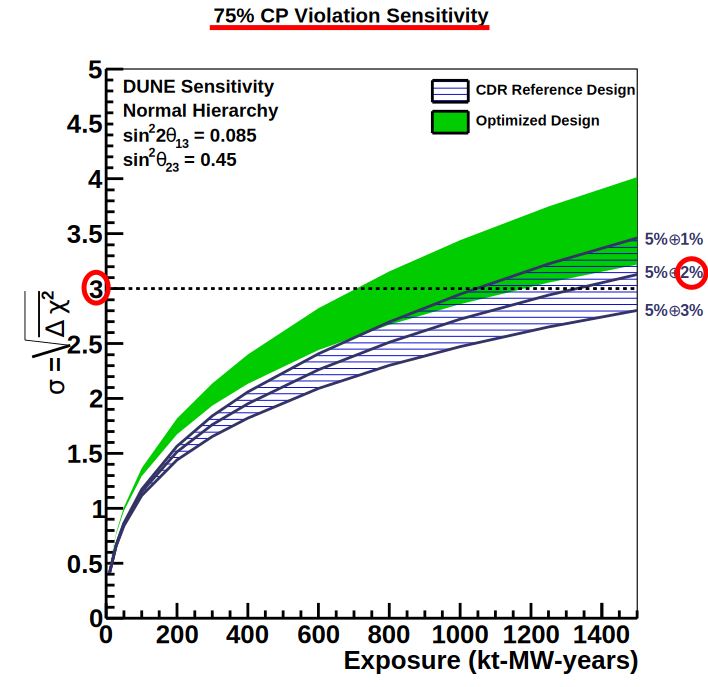
\includegraphics[width=\textwidth]{dune/cpv75_exp_syst}\\
		{\tiny \dune\ arXiv:~1512.06148~\cite{dune}}\\
		\num{25} years with \SI{40}{\kilo\tonne}\\
		{\color{\emphcol} $\Rightarrow$ need beam intensity $> \SI{1}{\mega\watt}$}\\
		\column{.5\textwidth}
		\SI{75}{\percent} CP violation coverage at $\num{3}\sigma$ requires beam related uncorrelated uncertainties $< \SI{2}{\percent}$.\\
		{\color{\emphcol} Constraining beam at near detector} requires
		\begin{itemize}
			\item High statistics
			\item High resolution
			\item[$\Rightarrow$] Good background rejection
			\item Ideally, same material and technology as far detector
			\item[$\Rightarrow$] Cancel uncertainties on
			\begin{itemize}
				\item Cross section
				\item Detector response
			\end{itemize}
		\end{itemize}
	\end{columns}
\end{frame}

\begin{frame}{Challenges for the near detector}{High energies and multiplicities}
	\begin{itemize}
		\item Simluation of a single neutrino beam spill, including backgrounds
		\item {\color{\emphcol} \num{0.2} beam events per tonne @ \SI{2}{\mega\watt}}
	\end{itemize}
	\centering
	\includegraphics[height=.6\textheight]{defence/dune_nd_pile-up}\\
	{\tiny \SI{200}{\tonne} LAr near detector, James Sinclair, University of Bern, 2016}\\
\end{frame}

\begin{frame}{The time projection chamber (TPC)}{A detector providing precise tracking and calorimetry}
	\centering
	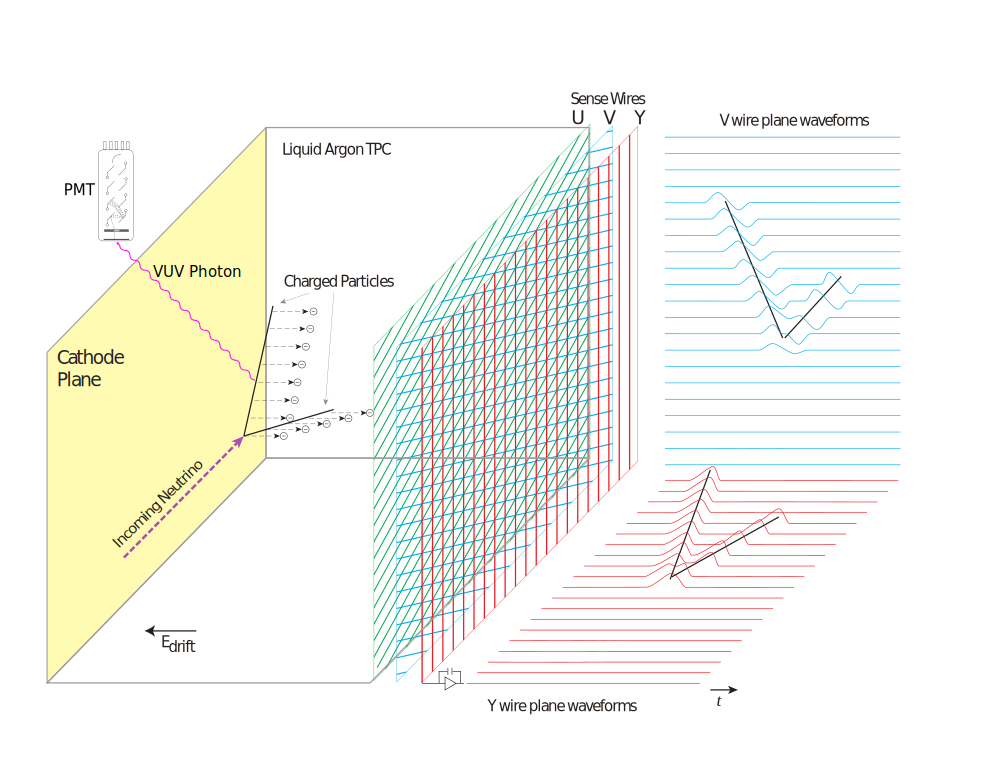
\includegraphics[viewport=35 40 720 540, clip, height=.66\textheight]{defence/TPCprinciple}\\
	{\tiny \uboone{} arXiv:~1612.05824~\cite{uboone}}\\
\end{frame}

\section{Drift field generation}

\begin{frame}{The standard TPC design}{Drift field generation}
	\centering
	\includegraphics[viewport=35 40 720 540, clip, height=.66\textheight]{defence/TPCprinciple_HV}\\
	{\tiny \uboone{} arXiv:~1612.05824~\cite{uboone}}\\
\end{frame}

\section{Charge readout}

\begin{frame}{The standard TPC design}{Charge readout}
	\centering
	\includegraphics[viewport=35 40 755 540, clip, height=.66\textheight]{defence/TPCprinciple_charge-ro}\\
	{\tiny \uboone{} arXiv:~1612.05824~\cite{uboone}}\\
\end{frame}

\section{Light readout}

\begin{frame}{The standard TPC design}{Light readout}
	\centering
	\includegraphics[viewport=30 40 720 540, clip, height=.66\textheight]{defence/TPCprinciple_light-ro}\\
	{\tiny \uboone{} arXiv:~1612.05824~\cite{uboone}}\\
\end{frame}

\end{document}